\documentclass[18pt]{beamer}
\usepackage{templates/beamerthemekit}
\titlelogo{empty_logo}
\titleimage{KASCADE-img}

\title[Cosmic rays data center]{Current status of data center for cosmic rays \\based on KCDC}
\subtitle{GRID-2018, Dubna}
\author{\underline{Victoria Tokareva}, Dmitriy Kostunin}

\institute{Institute for Nuclear Physics (IKP)}

\date{September 12, 2018}

% Bibliography

\usepackage[citestyle=authoryear,bibstyle=numeric,hyperref,backend=biber]{biblatex}
\addbibresource{templates/example.bib}
\bibhang1em

\newcommand{\itemarrow}{\scriptsize\raise1.25pt\hbox{\textcolor{kit-green100}{$\blacktriangleright$}}}
\newcommand{\concl}[1]{\item[\itemarrow]\textcolor{kit-green100}{#1}}
\renewcommand{\thefootnote}{\fnsymbol{footnote}}
\newlength{\cellwidth}
\setlength{\cellwidth}{0.43\textwidth}
\newcommand{\cellbox}[1]{\parbox{\cellwidth}{\vspace{1ex}#1\vspace{1ex}}}

\begin{document}

% change the following line to "ngerman" for German style date and logos
\selectlanguage{english}

%INTRODUCTION

%title page
\begin{frame}
\titlepage
\end{frame}

\section{Introduction}

\begin{frame}{Big data in astroparticle physics (APP)}
    \small
    \begin{minipage}[c]{0.58\textwidth}
        \begin{center}
            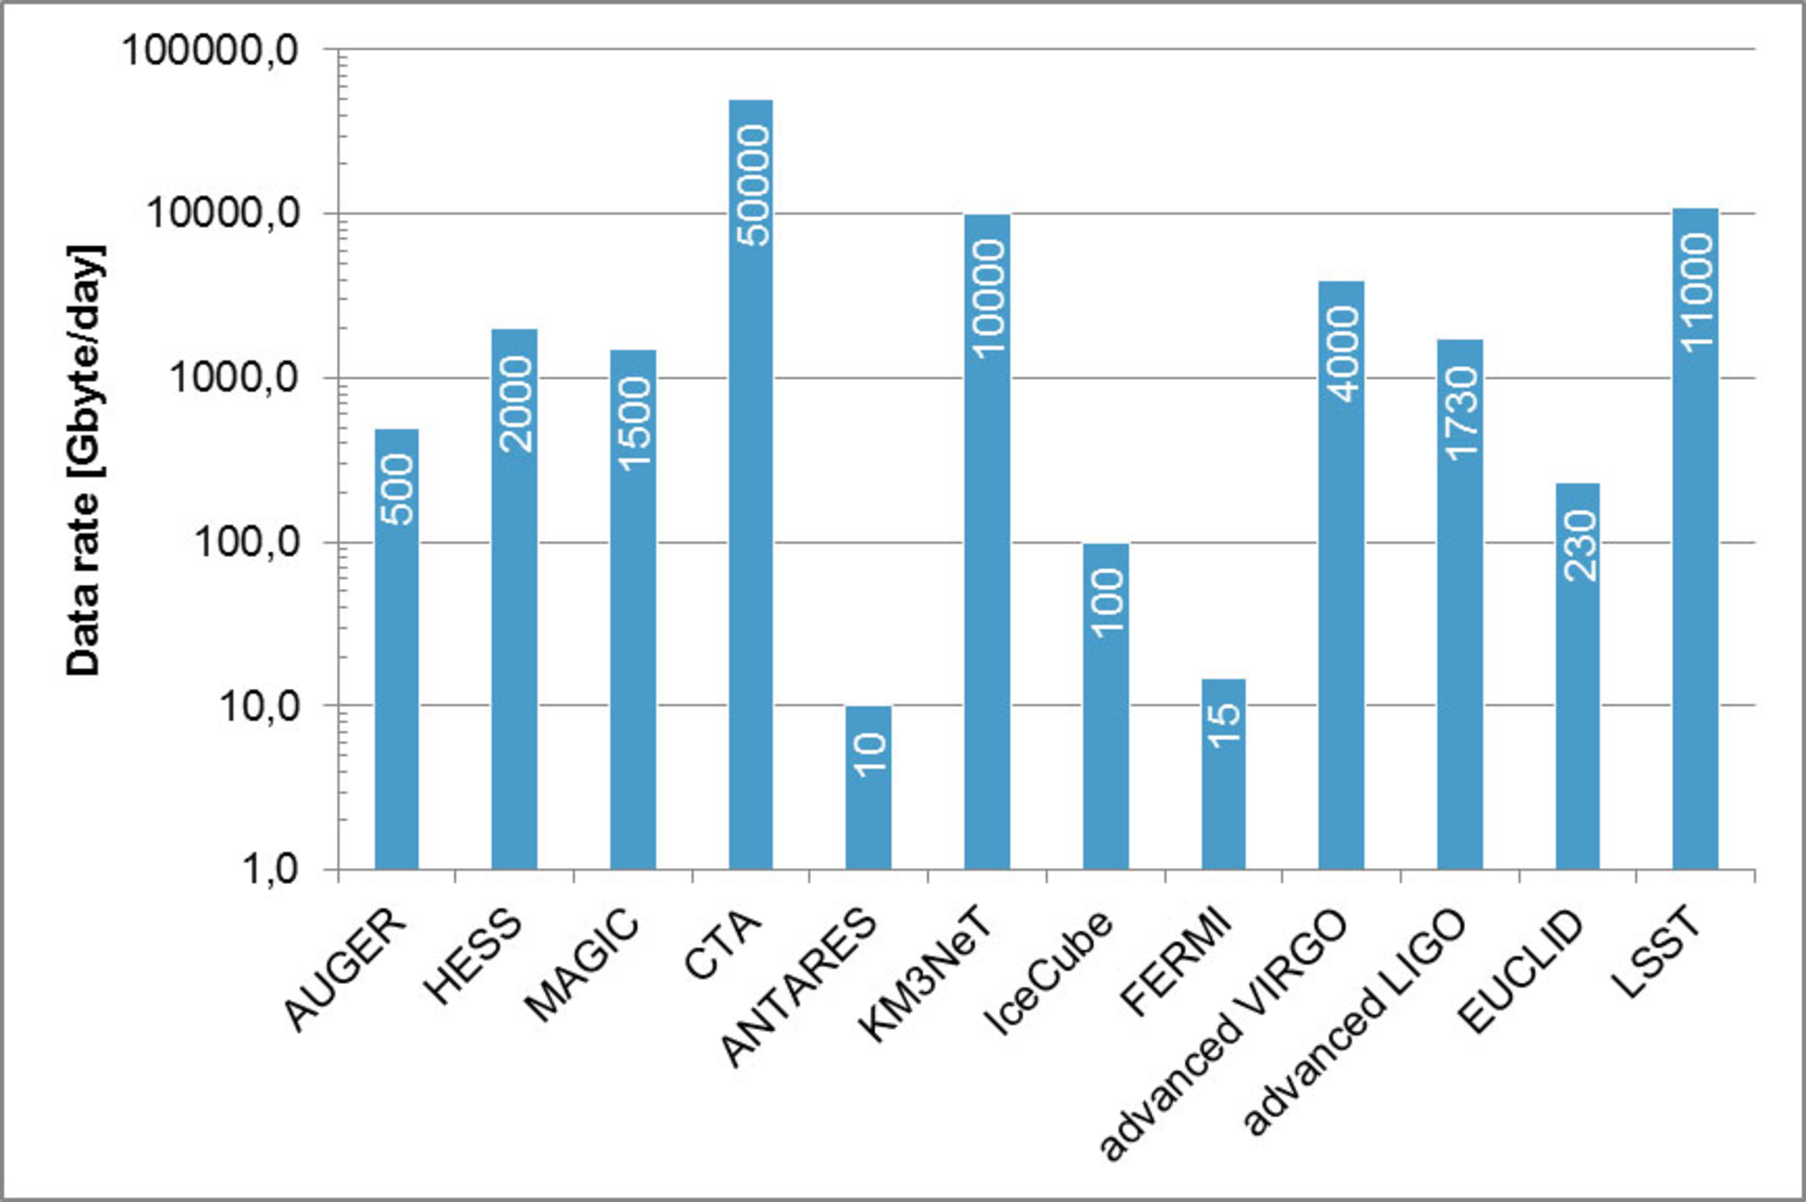
\includegraphics[width=1\textwidth]{pics/appec_computing-diagram.pdf}
        \end{center}
        \vspace{-2\parsep}
        \small Modern astroparticle experiments data rate [Gbytes/day]\footnotemark[1] %, source: APPEC brochure on Computing, 2016}
    \end{minipage}
    \hfill
    \begin{minipage}[c]{0.41\textwidth}
        \begin{itemize}
            \setlength{\itemsep}{0pt}
            \item Wide range of experiments;
            \item More than hundred years of cosmic particle measurements;
            \item Looking at the same sky with different detectors;
            \item Common data rate for astroparticle physics experiments all together is a few PBytes/year, which is comparable to the current LHC output\footnotemark[1]
            \item Big data for deep learning
        \end{itemize}
    \end{minipage}
    \footnotesize\footnotetext[1]{Berghöfer T., Agrafioti I. et all. Towards a model for computing in European astroparticle physics, Astroparticle Physics European Coordination committee, 2016}
\end{frame}

\begin{frame}{Software data life cycles}% and information management
    \begin{itemize}
        \item \textbf{Data engineering} includes development and support of data architecture and a data pipeline for a platform that enables data analysts, scientists, and other personnel to query the data.
        % and organization and support of a data pipeline that connects all the pieces of the data ecosystem together.
        
        \item \textbf{Data Life Cycle (DLC)} is the sequence of stages that a particular unit of data goes through from its initial generation 
        or capture to its eventual archival and/or deletion. The typical data life cycle includes data gathering, processing, storage, analysis, sharing and archiving. 
        % The data life cycle provides a high level overview of the stages involved in successful management and preservation of data for use and reuse.

        % \item \textbf{Data engineering} includes development of the architecture for a data platform that enables data analysts, scientists, and other curious 
        %  types to query their data and organization and support of a data pipeline that connects all the pieces of the data ecosystem together.
        %  
        %  \item \textbf{Data Life Cyce (DLC)} is the sequence of stages that a particular unit of data goes through from its initial generation 
        % or capture to its eventual archival and/or deletion. The typical data life cycle includes data gathering, processing, storage, analysis, sharing and archiving. The data life cycle provides a high level overview of the stages involved in successful management and preservation of data for use and reuse.
    \end{itemize}
    \vspace{-1ex}
    \centering
    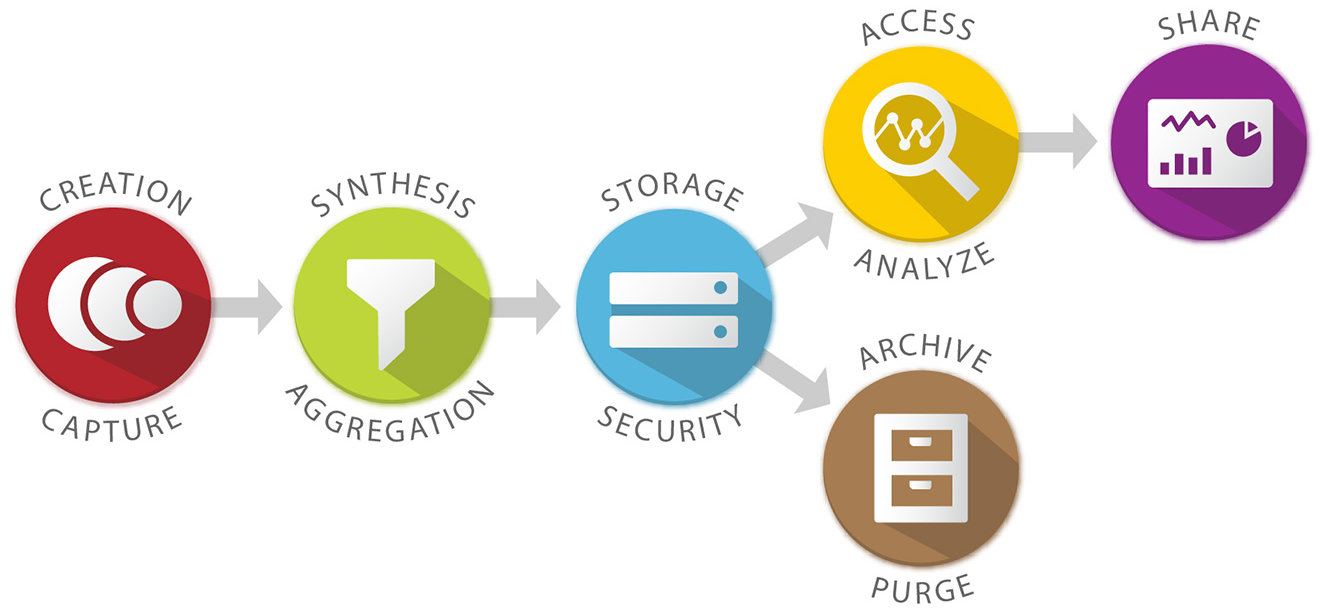
\includegraphics[width=0.65\textwidth]{pics/data_lifecycle_illust.jpg}
\end{frame}

%contents
\begin{frame}{Data engineering in APP}

\begin{minipage}[c]{0.52\textwidth}
\small
  \begin{itemize}
      \setlength{\itemsep}{0pt}
%       \item  Introduction \textcolor{kit-green100}{$\rightarrow$ we are here}
      \item  GRADLC initiative and main objectives
      \item  Features of DLC in APP
      \item  KASCADE Cosmic-ray Data Center
      \item  Proposed DLC architecture
      \item  Data aggregation server: metadata, data summary and workflows
%       \begin{itemize}
% 	  \item Metadata architecture
% 	  \item Data workflows 
% 	  \item Data summary and challenges (no slide so far :-( )
% 	  \item Possible solutions (postgres, cvmfs, etc...)
%       \end{itemize}
      \item   Application server: conception, computing sources and analysis
%       \begin{item}
% 	  \item conception 
% 	  \item computing sources
% 	  \item analysis 
% 	  \item possible solutions
%       \end{item}
      \item  Example: stacked analysis of high-energetic gamma rays
      \item  Outlook
%     \item  DCL in APP - specific
%     \item  DCL architecture
%     \item  Experiments and data specific
%     \item  Joint analysis scheme
%     \item  Possible solutions
%     \item  Outlook and future work
  \end{itemize}
\end{minipage}
\hfill
\begin{minipage}[c]{0.47\textwidth}
  
\includegraphics[width=1\textwidth]{pics/DE_fun.pdf}
\end{minipage}
\end{frame}

%GRADLC initiative descripton 

\begin{frame}{German-Russian Astroparticle \\Data Life Cycle Initiative\footnotemark[1]}
\vspace{-1.4em}
\begin{center}
  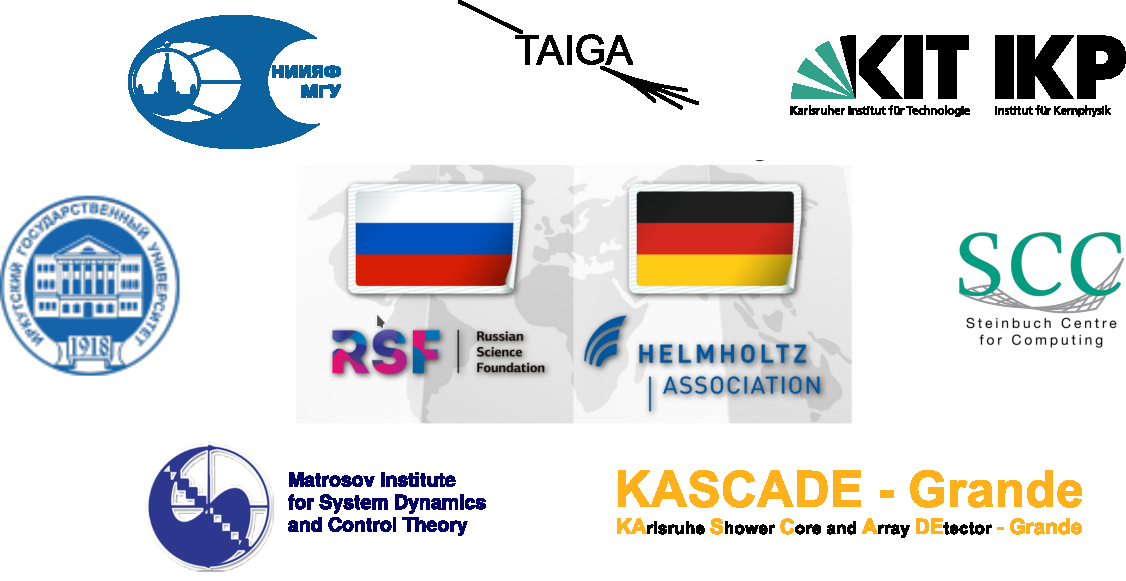
\includegraphics[width=0.9\textwidth]{pics/Collab-4.pdf}
\end{center}
\footnotesize\footnotetext[1]{Granted by RSF-Helmholtz Joint Research Groups}
\end{frame}

% %experiments overview

\begin{frame}{KASCADE-Grande}
\begin{itemize}
  \item Proposed in 1989---disassembled in 2013;
  \item Aimed at studying
  high-evergy (galactic) cosmic rays by observing extensive air showers (EAS);
%   processes at the edge of the Galaxy and beyond by observing extended atmospheric showers (EAS);
  \item Consisted of:
  \begin{itemize}
    \item scintillator arrays:
%     detecting $e$, $\gamma$, $\mu$:
    \begin{itemize}
  %сцинтиляторы, различают e, gamma, mu
    \item KASCADE---256 stations;
    \item GRANDE---37 stations;
    \end{itemize}
 %один большой калориметр
    \item Hadronic callorimeter;
 %радиодетектор
    \item Digital radio array LOPES;
%     detecting $e$, $e^{+}$;
% позволяющих наблюдать различные компоненты ливня
  \end{itemize}
  \item Important features of cosmic-ray spectrum have been obtained. The data analysis is ongoing;
%  благодаря данным с эксперимента было открыто много всего ополезного, при этом анлиз данных продолжается. новые статьи выходят
  \item KCDC (\textbf{K}ASCADE \textbf{C}osmic Ray \textbf{D}ata \textbf{C}enter, \textcolor{blue}{\texttt{http://kcdc.ikp.kit.edu}}) is a dedicated portal where all the data collected are available online. % At the moment
\end{itemize}

\begin{tikzpicture}[remember picture,overlay]
  \node[xshift=-12ex,yshift=-21ex] at (current page.north east){%
    
\includegraphics[width=0.3\textwidth]{pics/KCDC-Logo.png}
  };
\end{tikzpicture}
% \parbox[t][0pt]{0pt}{
%   \vspace{-0.63\textheight}
%   ~\hspace{0.68\textwidth}
\includegraphics[width=0.3\textwidth]{pics/KCDC-Logo.png}
% }
\end{frame}

\begin{frame}{TAIGA - Tunka Advanced Instrument for cosmic ray physics and Gamma Astronomy}
% \footnotesize
% % \vspace{-1em}
\begin{itemize}
 \item The detectors construction started in 90s with Tunka-25 setup;
 \item Changed name from Tunka to TAIGA;
 \item Is ongoing and continiously enhancend;
%  \item Currently consists of 4 detectors presented + TUNKA IACT is under construction;
\end{itemize}

% \vspace{2em}

\begin{center}
    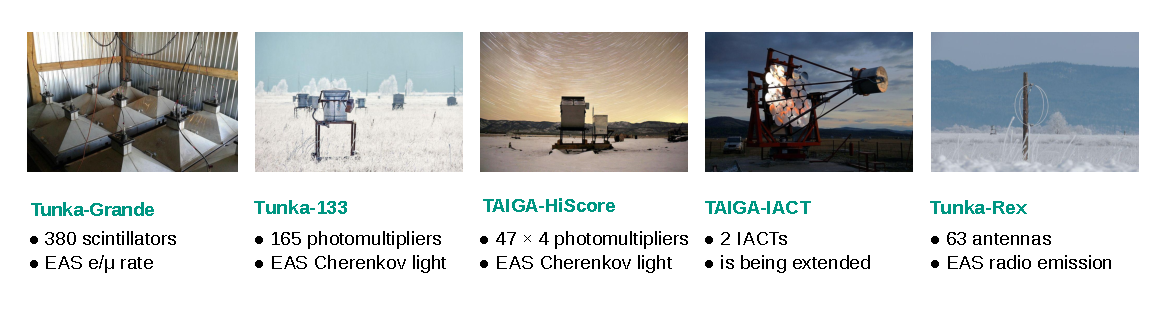
\includegraphics[width=1\textwidth]{pics/TAIGA_exp_wt.pdf} 
\end{center}

\end{frame}

 - experiments overview. Is not requiered is this IT=specified presentation
% 
% \begin{frame}{The main objectives}
% \begin{minipage}[c]{0.45\textwidth}
%   \begin{itemize}
%     \item  Provide sustainable access to scientific data
%     \item  Archiving of Data and Metadata
%     \item  Providing analysis tools
%     \item  Education in Big Data Science
%   \end{itemize}
% \end{minipage}
% \hfill
% \begin{minipage}[c]{0.54\textwidth}
%   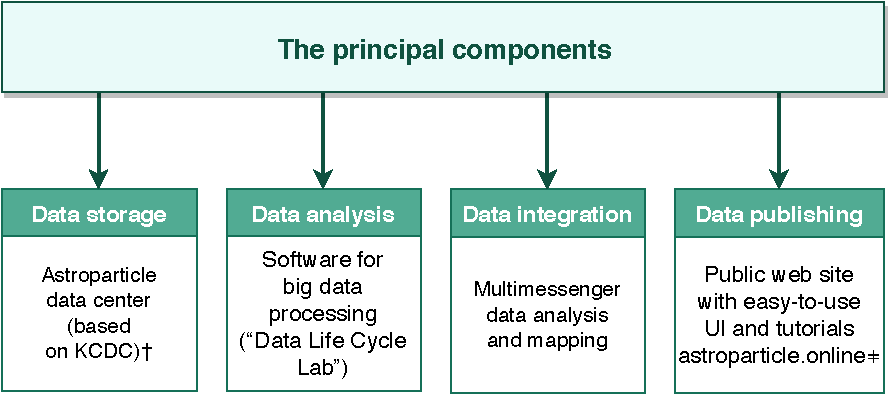
\includegraphics[width=1\textwidth]{pics/proj_objectives.pdf}
% \end{minipage}
%   \vspace{-\topsep}
%   \vspace{-\partopsep}
%   \vspace{\itemsep}
%   \vspace{\parsep}
%   \begin{itemize}
%     \item  Development area for multi-messenger analyses (e.g. Deep Learning)
%     \item  Platform for communication and exchange within Astroparticle Physics
%   \end{itemize}
% \end{frame}
% 



% \section{The project objectives}
\section{The data integration approach}

\begin{frame}{The project objectives}
% Work packages:

\vspace{-1em}
\begin{center}
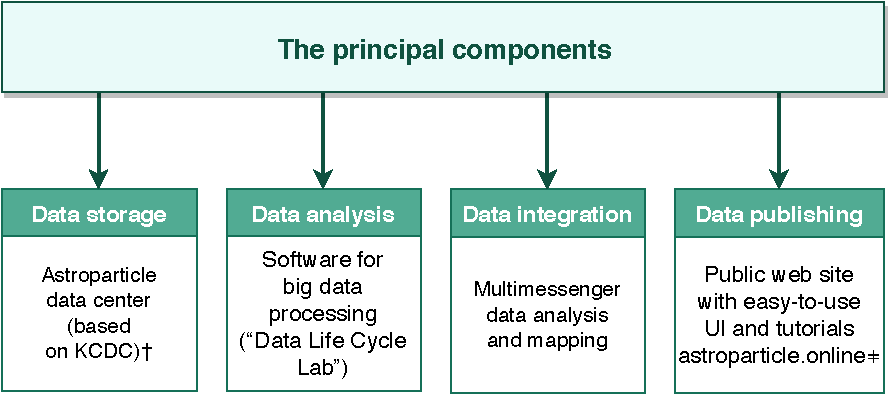
\includegraphics[width=0.82\textwidth]{pics/proj_objectives.pdf}
\end{center}

%   \item Minh Duc Nguyen, \textit{A distributed data warehouse system for astroparticle physics}, GRID2018 session 10
%   \item Yu. Kazarina, \textit{Application of Hubzero platform for the educational process in astroparticle physics}, GRID2018 poster

\footnotesize\footnotetext[2]{Minh Duc Nguyen, \textit{A distributed data warehouse system for astroparticle physics}, GRID2018 session 10}
\footnotesize\footnotetext[3]{Yu. Kazarina, \textit{Application of Hubzero platform for the educational process in astroparticle physics}, GRID2018 poster}
%proj_objectives.png
% \textcolor{red}{Add the 'data flow' scheme!!!}
% \begin{itemize}
%  \item Astroparticle data center (based on KCDC)
%  \item Software for big data processing (“Data Life Cycle Lab”)
%  \item Multimessenger data analysis and mapping
%  \item Go for the public ( astroparticle.online )
% \end{itemize}
\end{frame}

\begin{frame}{Deep into KASCADE and Tunka data formats}
\vspace{-2em}
\begin{minipage}[t]{0.48\textwidth}
  \begin{block}{Different}
    \begin{itemize}
      \item Data format (depends on avalilable detectors)
%         \item Information on detector properties (e.g.\ calibrations)
      \item Dedicated software for analyzing data
      \item Special system environment for the software
    \end{itemize}
  \end{block}
\end{minipage}
\hfill
\begin{minipage}[t]{0.48\textwidth}
  \begin{block}{Common}
    \begin{itemize}
      \item Metadata format (e.g.\ time, location, atmospheric conditions)
      \item Software for EAS simulation (e.g. CORSIKA)
      \item Shower parameters
      \item Theoretical models
    \end{itemize}
  \end{block}
\end{minipage}

%  \begin{exampleblock}{title}
%   text
%  \end{exampleblock}

\begin{minipage}[t]{0.48\textwidth}
  \begin{exampleblock}{Current state}
    \begin{itemize}
      \item Separate APIs and UIs for different experiments
    \end{itemize}
  \end{exampleblock}
\end{minipage}
\hfill
\begin{minipage}[t]{0.48\textwidth}
  \begin{exampleblock}{Our objective}
    \begin{itemize}
      \item Unified API and UIs for different experiments
    \end{itemize}
  \end{exampleblock}
\end{minipage}
\end{frame}

\begin{frame}{WMS---workload management system}
% \textcolor{red}{\textit{Taken from Petrosyan's talk}}
\begin{itemize}
  \item The basic idea is to provide a central queue for all users and make all the distributed sites look like local ones;
  \item Starting from mid 90's are widely used in collider experiments (AliEn, Dirac, PanDA);
  \item Dedicated for:
  \begin{itemize}
  \item Unified usage of the distributed remote data and common data analysis;
  \item Conceal various low-level software and provide unified high-level interface;
  \end{itemize}
%   \item
%   Hide middleware while supporting diversity and evolution
%   \begin{itemize}
%     \item WMS interacts with middleware, users see only high level workflow
%     \item Automation engines built in WMS, not exposed to users
%   \end{itemize}
  \item Provide the common way to issue tasks to different types of the distibuted sites;
  \item
%   Use the same system for simulation, data processing and users analysis
  The same system for the data access, analysis and simulation.
%   \item Similar ideas have been implemented in several independent systems developed by LHC experiments: AliEn, Dirac, PanDA
\end{itemize}
\end{frame}

\begin{frame}{Data-oriented approach}
% \vspace{-1em}
What data do we work with?

% \vspace{3em}

\parbox{0.48\textwidth}{
\begin{itemize}
  \item Data types:
  \begin{itemize}
    \item Raw detector readouts;
    \item Pre-analyzed events;
    \item Metadata
  \end{itemize}
\end{itemize}
}
\hfill
\parbox{0.48\textwidth}{
\begin{itemize}
  \item Data structure:
  \begin{itemize}
    \item Different formats;
    \item Different messengers;
    \item Common metadata
  \end{itemize}
\end{itemize}
}

Our approach:
\begin{itemize}
 \item It is proposed to store unique event id and metadata in the unified database
 \item With growing data sizes, distribured storage for events could be useful
\end{itemize}
\end{frame}

% \begin{tabular*}{1\textwidth}{p{0.45\textwidth}@{\extracolsep{\fill}}p{0.45\textwidth}}
% \hline\multicolumn{2}{c}{Location} \\
% % Experiments: remote locations with no or limited internet access &
% % Servers: data are transferred periodically on tapes or disks \\
% % \hline\multicolumn{2}{c}{Data} \\
% % Raw detector readouts: analyzed offline, not stored &
% % Pre-analyzed events: stored on servers \\
% % \hline\multicolumn{2}{c}{Different \& common} \\
% % Each experiment has its own detectors and provides its own format of events &
% % Events share \emph{common metadata} (e.g.\ time, location, atmospheric conditions) \\
% \hline\multicolumn{2}{c}{Storage} \\
% It is proposed to store unique event id and metadata in the unified database &
% With growing data sizes, distribured storage for events could be useful \\
% \hline
% \end{tabular*}

% \begin{frame}{Data storage}
% \begin{itemize}
%   \item Some experiments (in our case, TUNKA) are situated at remote locations with no or limited internet access, raw data are transferred periodically to servers on tapes or disks
%   \item Raw data are pre-analyzed, so-called ``direct'' observables ($e$, $\mu$, $\gamma$, $\hat{C}$, radio, etc.) are obtained, events are stored on servers
%   \item Each experiment has its own detectors and provides its own format of events
%   \item Events share \emph{common metadata} (e.g.\ time, location, atmospheric conditions)
%   \item It is proposed to store unique event id and metadata in the unified database
%   \item With growing data sizes, distribured storage for events could be useful
% \end{itemize}
% \end{frame}

\begin{frame}{Proposed cosmic-ray metadata structure}
\vspace{-1.5em}
\begin{center}
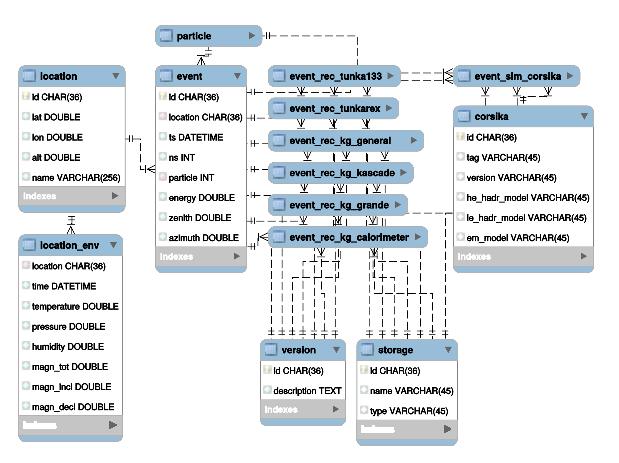
\includegraphics[width=0.82\textwidth]{pics/metadata.eps}
\end{center}
\end{frame}

\begin{frame}{Data analysis}
\begin{itemize}
  \item Software for data analysis depends on a particular experiment
  \begin{itemize}
    \item Problem: It may even require dedicated system environment
    \concl{Solution: Virtualization could be useful}
  \end{itemize}
  \item Data analysis requires huge amounts of input data
  \begin{itemize}
    \item Problem: It is often more optimal to perform it on the same site the data are stored
    \concl{Solution: Job management could handle the task}
  \end{itemize}
\end{itemize}
\end{frame}

\begin{frame}{Simulation}
\centering
\begin{tabular*}{1\textwidth}{c@{~~~$\Rightarrow$~~~}c}
\multicolumn{1}{c}{\textbf{Feature}} &
\multicolumn{1}{c}{\textbf{Consequence}} \\ \hline
\cellbox{The software for EAS simulation (e.g.\ CORSIKA) does not depend on a particular experiment} &
\cellbox{Simulations require standartized system environment} \\
\cellbox{
  Simulations require small amounts of input data

  Simulations can be done independently for different events
} &
\cellbox{Simulations are easily scalable} \\
\cellbox{Simulations require a lot of computing resources} &
\cellbox{HPC sites are needed} \\ \hline
\end{tabular*}

\vspace{1ex}
\centering\textbf{\textcolor{kit-green100}{Distributed computing could be useful}} \\
\end{frame}

\begin{frame}{Distributed analysis and simulation scheme}
% \textcolor{red}{Схема~--- проверить!)}
\vspace{-1em}
\begin{center}
% 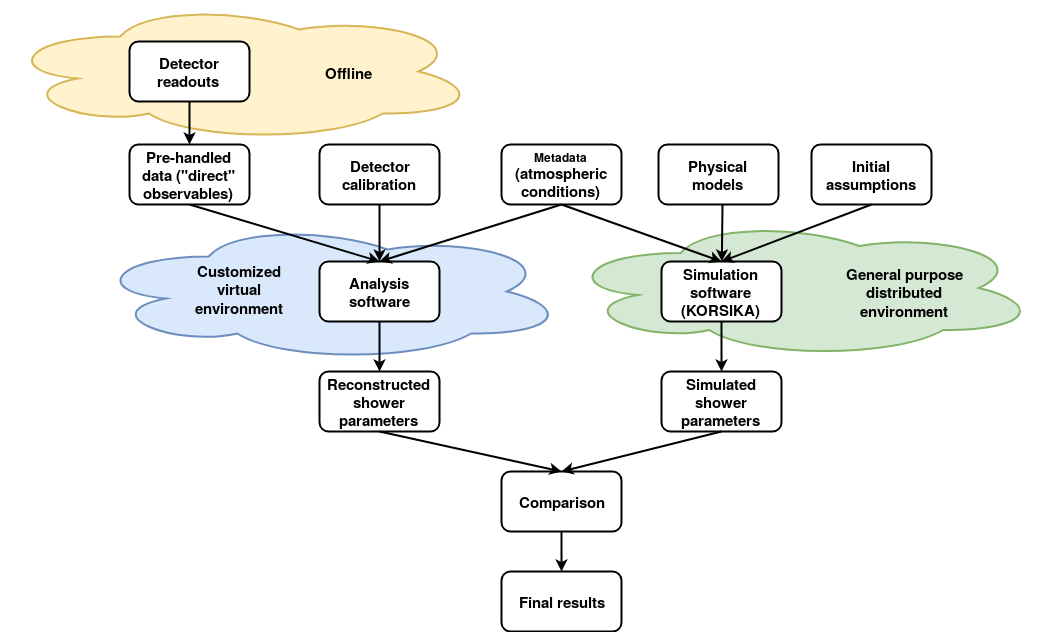
\includegraphics[width=0.85\textwidth]{pics/KCDC_workflow_f1.png}
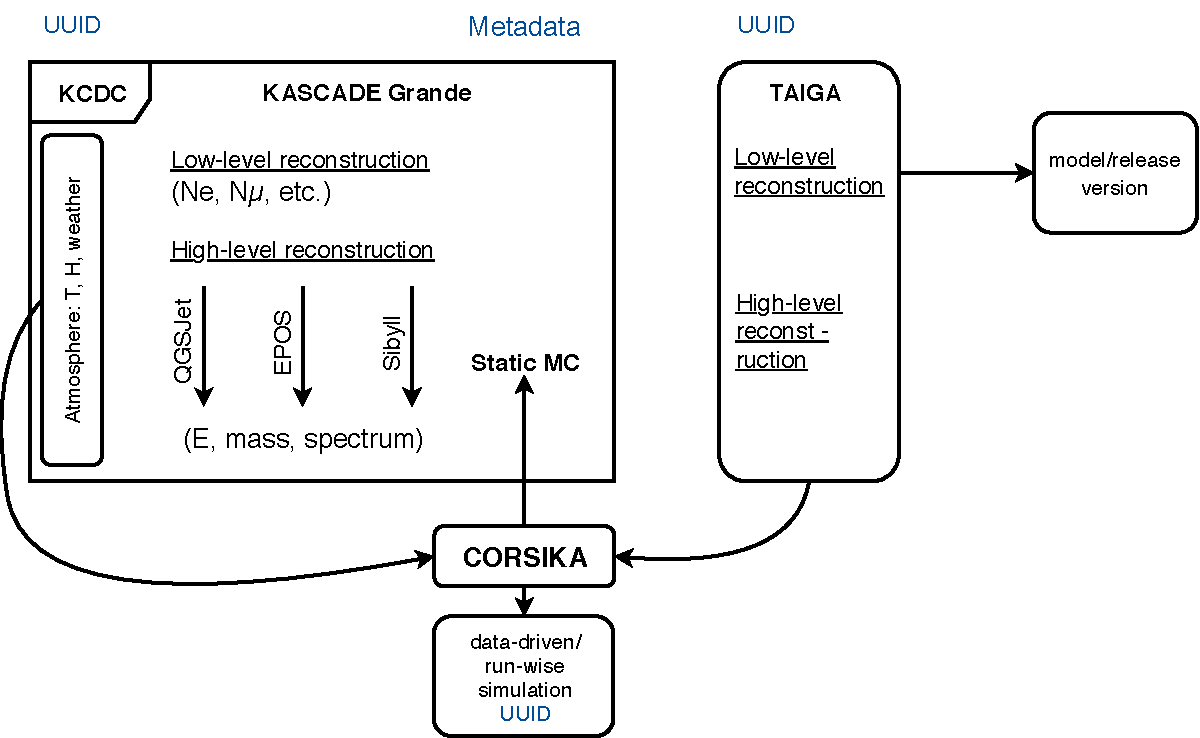
\includegraphics[width=0.85\textwidth]{pics/kcdc_scheme_k.pdf}
\end{center}
\end{frame}

% \begin{frame}{Mapping of observables between experiments}
%
% \textcolor{red}{Draw the sheme of the mapping!!! See the Kostunin's slide \#8}
%
% \begin{block}{Draft}
%   \begin{itemize}
%     \item Calibrations provided by experiments
%     \item Various models
%     \item Implementations are stored
%   \end{itemize}
% \end{block}
% \begin{center}
%   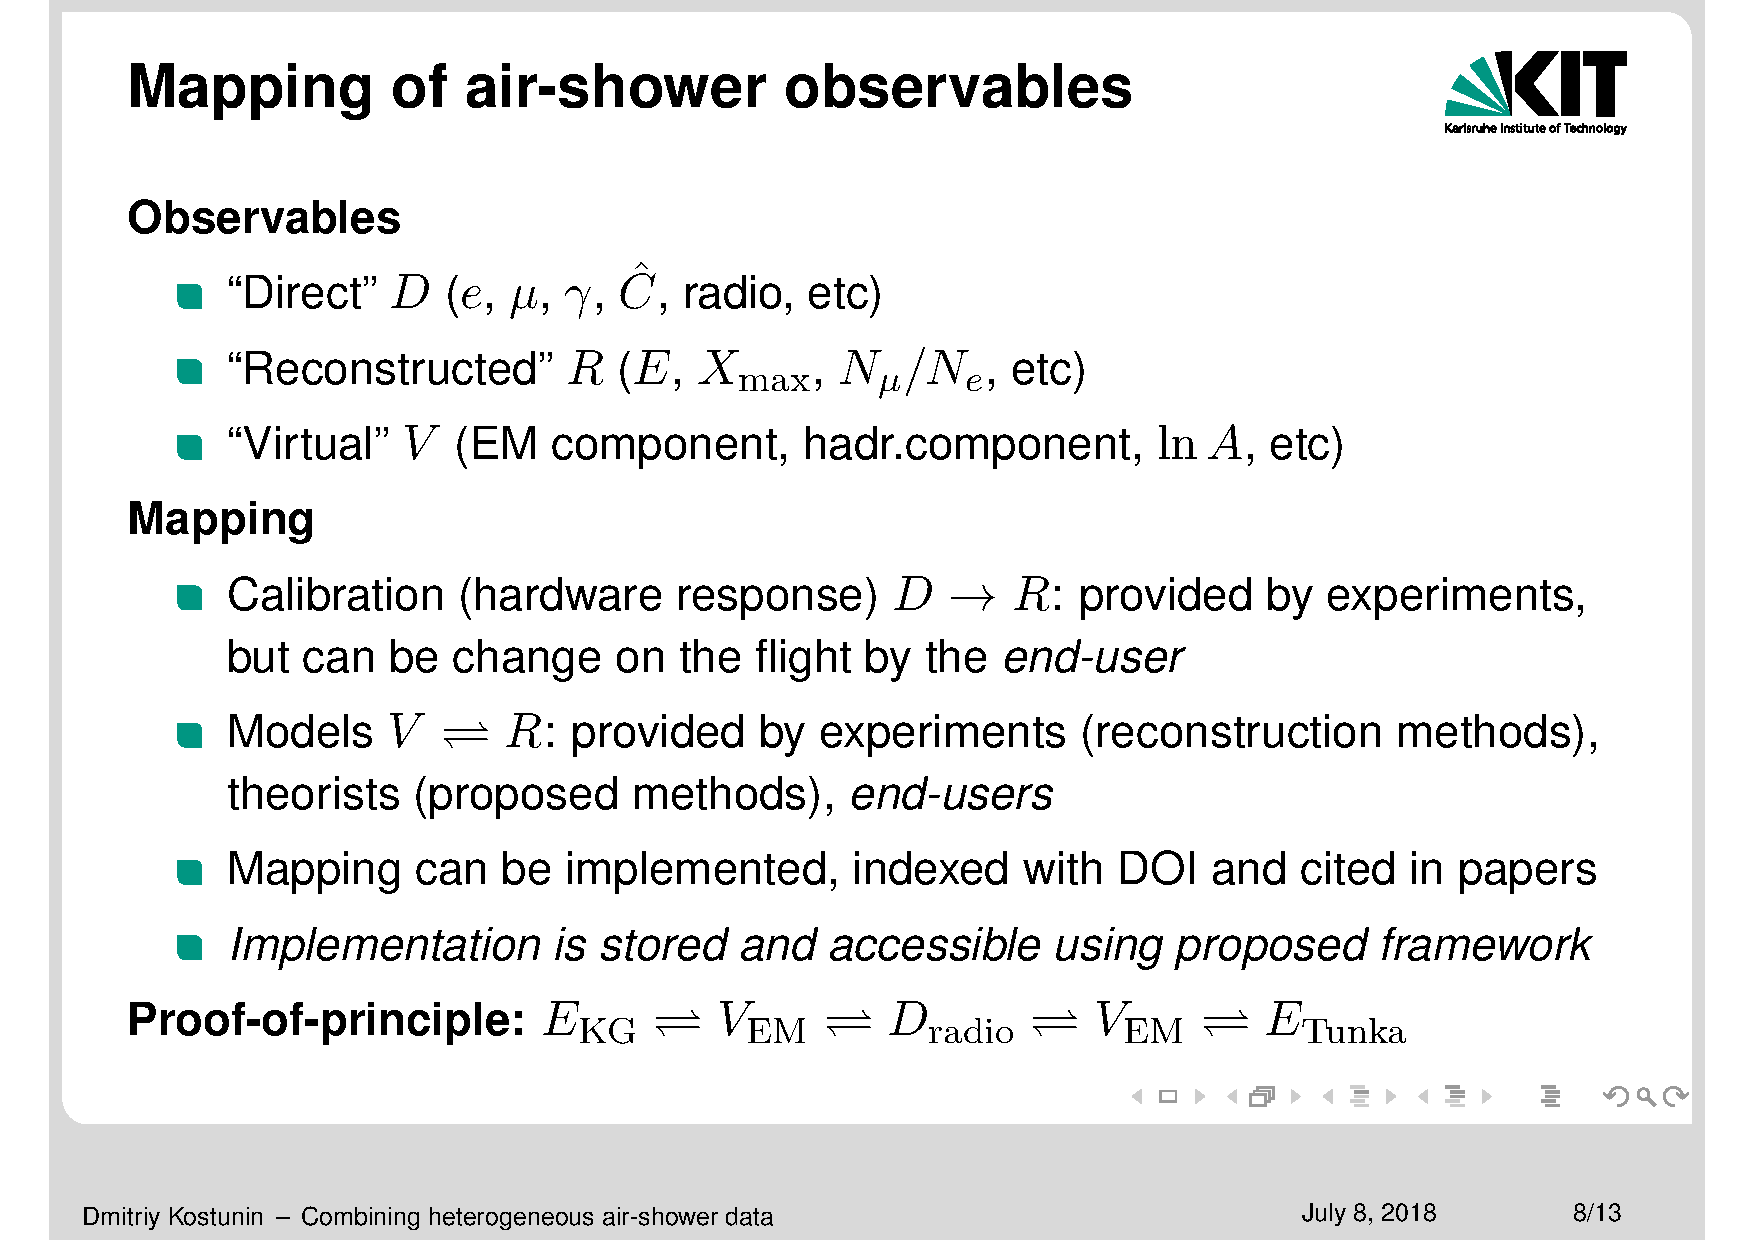
\includegraphics[width=0.7\textwidth]{pics/k8.pdf}
% \end{center}
% \end{frame}

% \begin{frame}{Access}
% \begin{block}{Draft}
%   \begin{itemize}
%     \item Benefits of open access
%     \item Education and outreach
%     \item Which infrastructure to use?
%   \end{itemize}
% \end{block}
% \end{frame}

% %CONCLUSION
\section{Conclusion}

% \begin{frame}{Open access and education}
%     \vspace{-4em}
%     \begin{itemize}
%         \item Open access: a dedicated portal planned
%         \item Education: \textcolor{blue}{\texttt{astroparticle.online}}
%     \end{itemize}
%     \centering
%     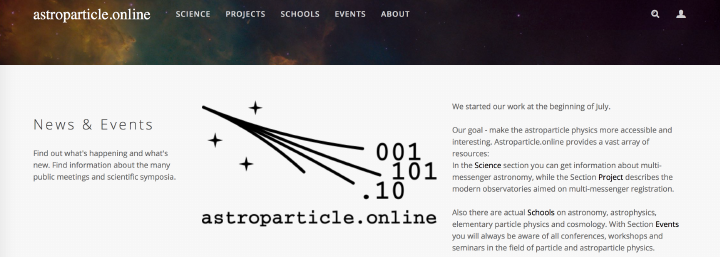
\includegraphics[width=0.85\textwidth]{pics/astro_onl.png}
% \end{frame}

\begin{frame}{Outlook}
% \textcolor{red}{Improve the translation quality!!!}
\begin{itemize}
\item Done so far:
    \begin{itemize}
    \item Metadata DB filled out with sample data of KASCADE and Tunka-133;
    \item The filling with the main amount is ongoing;
    \end{itemize}
\item ToDo: 
    \begin{itemize}
     \item Metadata extractor for KCDC;
    \end{itemize}

\item Open for discussion:
\begin{itemize}
 \item 2nd level MD search - the place in the general scheme;
 \item user interface;
 \item data mapping;
\end{itemize}

 \end{itemize}
\end{frame}

% \subsection{The end}
% \begin{frame}{}
%     \begin{center}
%         \textcolor{kit-green100}{\Huge Thank you\\for your attention!\vspace{1em}}  
%         \Large Any questions?
%     \end{center}
% \end{frame}


% \appendix
% \beginbackup
%
% \begin{frame}[allowframebreaks]{References}
% \printbibliography
% \end{frame}
%
% \backupend

\end{document}
